\documentclass{anstrans}
%%%%%%%%%%%%%%%%%%%%%%%%%%%%%%%%%%%
\title{FIXME: Abstract Title}
\author{FIXME: Authors}

\institute{
Dept. of Nuclear, Plasma and Radiological Engineering, University of Illinois at Urbana-Champaign \\
FIXME: Your email
}

%%%% packages and definitions (optional)
\usepackage{graphicx} % allows inclusion of graphics
\graphicspath{{./figures/}}
\usepackage{float}
\usepackage{booktabs} % nice rules (thick lines) for tables
\usepackage{microtype} % improves typography for PDF
\usepackage{xspace}
\usepackage{tabularx}
\usepackage{amsmath}
\usepackage{subcaption}
\usepackage{enumitem}
\usepackage{placeins}
\usepackage{tikz}
\usetikzlibrary{shapes.geometric, arrows}
\usepackage[acronym,toc]{glossaries}
%\newacronym{<++>}{<++>}{<++>}
\newacronym[longplural={metric tons of heavy metal}]{MTHM}{MTHM}{metric ton of heavy metal}
\newacronym{ABM}{ABM}{agent-based modeling}
\newacronym{ACDIS}{ACDIS}{Program in Arms Control \& Domestic and International Security}
\newacronym{ADS}{ADS}{Accelerator-Driven System}
\newacronym{AFCI}{AFCI}{Advanced Fuel Cycles Initiative}
\newacronym{AHTR}{AHTR}{Advanced High Temperature Reactor}
\newacronym{ANDRA}{ANDRA}{Agence Nationale pour la gestion des D\'echets RAdioactifs, the French National Agency for Radioactive Waste Management}
\newacronym{ANL}{ANL}{Argonne National Laboratory}
\newacronym{ANS}{ANS}{American Nuclear Society}
\newacronym{API}{API}{application programming interface}
\newacronym{app}{APP}{Abbott Power Plant}
\newacronym{ARE}{ARE}{Aircraft Reactor Experiment}
\newacronym{ARFC}{ARFC}{Advanced Reactors and Fuel Cycles}
\newacronym{ASME}{ASME}{American Society of Mechanical Engineers}
\newacronym{ASTRID}{ASTRID}{Advanced Sodium Technological Reactor for Industrial Demonstration}
\newacronym{ATWS}{ATWS}{Anticipated Transient Without Scram}
\newacronym{BDBE}{BDBE}{Beyond Design Basis Event}
\newacronym{BIDS}{BIDS}{Berkeley Institute for Data Science}
\newacronym{BWR}{BWR}{Boiling Water Reactor}
\newacronym{CAFCA}{CAFCA}{ Code for Advanced Fuel Cycles Assessment }
\newacronym{CDTN}{CDTN}{Centro de Desenvolvimento da Tecnologia Nuclear}
\newacronym{CEA}{CEA}{Commissariat \`a l'\'Energie Atomique et aux \'Energies Alternatives}
\newacronym{CI}{CI}{continuous integration}
\newacronym{CNEN}{CNEN}{Comiss\~{a}o Nacional de Energia Nuclear}
\newacronym{CNERG}{CNERG}{Computational Nuclear Engineering Research Group}
\newacronym{COSI}{COSI}{Commelini-Sicard}
\newacronym{COTS}{COTS}{commercial, off-the-shelf}
\newacronym{CSNF}{CSNF}{commercial spent nuclear fuel}
\newacronym{CTAH}{CTAHs}{Coiled Tube Air Heaters}
\newacronym{CUBIT}{CUBIT}{CUBIT Geometry and Mesh Generation Toolkit}
\newacronym{CURIE}{CURIE}{Centralized Used Fuel Resource for Information Exchange}
\newacronym{DAG}{DAG}{directed acyclic graph}
\newacronym{DANESS}{DANESS}{Dynamic Analysis of Nuclear Energy System Strategies}
\newacronym{DBE}{DBE}{Design Basis Event}
\newacronym{DESAE}{DESAE}{Dynamic Analysis of Nuclear Energy Systems Strategies}
\newacronym{DHS}{DHS}{Department of Homeland Security}
\newacronym{DOE}{DOE}{Department of Energy}
\newacronym{DRACS}{DRACS}{Direct Reactor Auxiliary Cooling System}
\newacronym{DRE}{DRE}{dynamic resource exchange}
\newacronym{DSNF}{DSNF}{DOE spent nuclear fuel}
\newacronym{DYMOND}{DYMOND}{Dynamic Model of Nuclear Development }
\newacronym{EBS}{EBS}{Engineered Barrier System}
\newacronym{EDF}{EDF}{Électricité de France}
\newacronym{EDZ}{EDZ}{Excavation Disturbed Zone}
\newacronym{EIA}{EIA}{U.S. Energy Information Administration}
\newacronym{EPA}{EPA}{Environmental Protection Agency}
\newacronym{EPR}{EPR}{European Pressurized Reactor}
\newacronym{EP}{EP}{Engineering Physics}
\newacronym{esom}{ESOM}{energy system optimization model}
\newacronym{EU}{EU}{European Union}
\newacronym{FCO}{FCO}{Fuel Cycle Options}
\newacronym{FCT}{FCT}{Fuel Cycle Technology}
\newacronym{FEHM}{FEHM}{Finite Element Heat and Mass Transfer}
\newacronym{FEPs}{FEPs}{Features, Events, and Processes}
\newacronym{FHR}{FHR}{Fluoride-Salt-Cooled High-Temperature Reactor}
\newacronym{FLiBe}{FLiBe}{Fluoride-Lithium-Beryllium}
\newacronym{FP}{FP}{Fission Products}
\newacronym{hsj}{HSJ}{Hop-Skip-Jump}
\newacronym{GDSE}{GDSE}{Generic Disposal System Environment}
\newacronym{GDSM}{GDSM}{Generic Disposal System Model}
\newacronym{GENIUSv1}{GENIUSv1}{Global Evaluation of Nuclear Infrastructure Utilization Scenarios, Version 1}
\newacronym{GENIUSv2}{GENIUSv2}{Global Evaluation of Nuclear Infrastructure Utilization Scenarios, Version 2}
\newacronym{GENIUS}{GENIUS}{Global Evaluation of Nuclear Infrastructure Utilization Scenarios}
\newacronym{GPAM}{GPAM}{Generic Performance Assessment Model}
\newacronym{GRSAC}{GRSAC}{Graphite Reactor Severe Accident Code}
\newacronym{GUI}{GUI}{graphical user interface}
\newacronym{HLW}{HLW}{high level waste}
\newacronym{HPC}{HPC}{high-performance computing}
\newacronym{HTC}{HTC}{high-throughput computing}
\newacronym{HTGR}{HTGR}{High Temperature Gas-Cooled Reactor}
\newacronym{IAEA}{IAEA}{International Atomic Energy Agency}
\newacronym{icap}{iCAP}{Illinois Climate Action Plan}
\newacronym{IEMA}{IEMA}{Illinois Emergency Mangament Agency}
\newacronym{IHLRWM}{IHLRWM}{International High Level Radioactive Waste Management}
\newacronym{INL}{INL}{Idaho National Laboratory}
\newacronym{IPRR1}{IRP-R1}{Instituto de Pesquisas Radioativas Reator 1}
\newacronym{IRP}{IRP}{Integrated Research Project}
\newacronym{ISFSI}{ISFSI}{Independent Spent Fuel Storage Installation}
\newacronym{ISRG}{ISRG}{Independent Student Research Group}
\newacronym{JFNK}{JFNK}{Jacobian-Free Newton Krylov}
\newacronym{LANL}{LANL}{Los Alamos National Laboratory}
\newacronym{LBNL}{LBNL}{Lawrence Berkeley National Laboratory}
\newacronym{LCOE}{LCOE}{levelized cost of electricity}
\newacronym{LDRD}{LDRD}{laboratory directed research and development}
\newacronym{LFR}{LFR}{Lead-Cooled Fast Reactor}
\newacronym{LLNL}{LLNL}{Lawrence Livermore National Laboratory}
\newacronym{LMFBR}{LMFBR}{Liquid Metal Fast Breeder Reactor}
\newacronym{LOFC}{LOFC}{Loss of Forced Cooling}
\newacronym{LOHS}{LOHS}{Loss of Heat Sink}
\newacronym{LOLA}{LOLA}{Loss of Large Area}
\newacronym{LP}{LP}{linear program}
\newacronym{LWR}{LWR}{Light Water Reactor}
\newacronym{MAGNOX}{MAGNOX}{Magnesium Alloy Graphie Moderated Gas Cooled Uranium Oxide Reactor}
\newacronym{MA}{MA}{minor actinide}
\newacronym{MCNP}{MCNP}{Monte Carlo N-Particle code}
\newacronym{mga}{MGA}{Modeling-to-Generate-Alternatives}
\newacronym{MILP}{MILP}{mixed-integer linear program}
\newacronym{MIT}{MIT}{the Massachusetts Institute of Technology}
\newacronym{MOAB}{MOAB}{Mesh-Oriented datABase}
\newacronym{MOOSE}{MOOSE}{Multiphysics Object-Oriented Simulation Environment}
\newacronym{MOX}{MOX}{Mixed Oxide Fuel}
\newacronym{MSBR}{MSBR}{Molten Salt Breeder Reactor}
\newacronym{MSRE}{MSRE}{Molten Salt Reactor Experiment}
\newacronym{MSR}{MSR}{Molten Salt Reactor}
\newacronym{MWe}{MWe}{Megawatts electric}
\newacronym{NAGRA}{NAGRA}{National Cooperative for the Disposal of Radioactive Waste}
\newacronym{NEAMS}{NEAMS}{Nuclear Engineering Advanced Modeling and Simulation}
\newacronym{NEUP}{NEUP}{Nuclear Energy University Programs}
\newacronym{NFCSim}{NFCSim}{Nuclear Fuel Cycle Simulator}
\newacronym{NGNP}{NGNP}{Next Generation Nuclear Plant}
\newacronym{NMWPC}{NMWPC}{Nuclear MW Per Capita}
\newacronym{NNSA}{NNSA}{National Nuclear Security Administration}
\newacronym{NPRE}{NPRE}{Department of Nuclear, Plasma, and Radiological Engineering}
\newacronym{NQA1}{NQA-1}{Nuclear Quality Assurance - 1}
\newacronym{NRC}{NRC}{Nuclear Regulatory Commission}
\newacronym{NSF}{NSF}{National Science Foundation}
\newacronym{NSSC}{NSSC}{Nuclear Science and Security Consortium}
\newacronym{NUWASTE}{NUWASTE}{Nuclear Waste Assessment System for Technical Evaluation}
\newacronym{NWF}{NWF}{Nuclear Waste Fund}
\newacronym{NWTRB}{NWTRB}{Nuclear Waste Technical Review Board}
\newacronym{OCRWM}{OCRWM}{Office of Civilian Radioactive Waste Management}
\newacronym{ORION}{ORION}{ORION}
\newacronym{ORNL}{ORNL}{Oak Ridge National Laboratory}
\newacronym{PARCS}{PARCS}{Purdue Advanced Reactor Core Simulator}
\newacronym{PBAHTR}{PB-AHTR}{Pebble Bed Advanced High Temperature Reactor}
\newacronym{PBFHR}{PB-FHR}{Pebble-Bed Fluoride-Salt-Cooled High-Temperature Reactor}
\newacronym{PEI}{PEI}{Peak Environmental Impact}
\newacronym{PHWR}{PHWR}{Pressurized Heavy Water Reactor}
\newacronym{PH}{PRONGHORN}{PRONGHORN}
\newacronym{ppa}{PPA}{power purchase agreement}
\newacronym{PRIS}{PRIS}{Power Reactor Information System}
\newacronym{PRKE}{PRKE}{Point Reactor Kinetics Equations}
\newacronym{PSPG}{PSPG}{Pressure-Stabilizing/Petrov-Galerkin}
\newacronym{PWAR}{PWAR}{Pratt and Whitney Aircraft Reactor}
\newacronym{PWR}{PWR}{Pressurized Water Reactor}
\newacronym{PyNE}{PyNE}{Python toolkit for Nuclear Engineering}
\newacronym{PyRK}{PyRK}{Python for Reactor Kinetics}
\newacronym{QA}{QA}{quality assurance}
\newacronym{RDD}{RD\&D}{Research Development and Demonstration}
\newacronym{RD}{R\&D}{Research and Development}
\newacronym{RELAP}{RELAP}{Reactor Excursion and Leak Analysis Program}
\newacronym{RIA}{RIA}{Reactivity Insertion Accident}
\newacronym{RIF}{RIF}{Region-Institution-Facility}
\newacronym{SFR}{SFR}{Sodium-Cooled Fast Reactor}
\newacronym{SINDAG}{SINDA{\textbackslash}G}{Systems Improved Numerical Differencing Analyzer $\backslash$ Gaski}
\newacronym{SKB}{SKB}{Svensk K\"{a}rnbr\"{a}nslehantering AB}
\newacronym{smr}{SMR}{small modular reactor}
\newacronym{SNF}{SNF}{spent nuclear fuel}
\newacronym{SNL}{SNL}{Sandia National Laboratory}
\newacronym{STC}{STC}{specific temperature change}
\newacronym{SUPG}{SUPG}{Streamline-Upwind/Petrov-Galerkin}
\newacronym{SWF}{SWF}{Separations and Waste Forms}
\newacronym{SWU}{SWU}{Separative Work Unit}
\newacronym{temoa}{Temoa}{Tools for Energy Model Optimization and Analysis}
\newacronym{TRIGA}{TRIGA}{Training Research Isotope General Atomic}
\newacronym{TRISO}{TRISO}{Tristructural Isotropic}
\newacronym{TSM}{TSM}{Total System Model}
\newacronym{TSPA}{TSPA}{Total System Performance Assessment for the Yucca Mountain License Application}
\newacronym{ThOX}{ThOX}{thorium oxide}
\newacronym{UFD}{UFD}{Used Fuel Disposition}
\newacronym{UML}{UML}{Unified Modeling Language}
\newacronym{UNF}{UNF}{Used Nuclear Fuel}
\newacronym{UOX}{UOX}{Uranium Oxide Fuel}
\newacronym{UQ}{UQ}{uncertainty quantification}
\newacronym{US}{US}{United States}
\newacronym{UW}{UW}{University of Wisconsin}
\newacronym{uiuc}{UIUC}{University of Illinois at Urbana-Champaign}
\newacronym{VISION}{VISION}{the Verifiable Fuel Cycle Simulation Model}
\newacronym{VVER}{VVER}{Voda-Vodyanoi Energetichesky Reaktor (Russian Pressurized Water Reactor)}
\newacronym{VV}{V\&V}{verification and validation}
\newacronym{WIPP}{WIPP}{Waste Isolation Pilot Plant}
\newacronym{YMR}{YMR}{Yucca Mountain Repository Site}

\makeglossaries

\newcolumntype{c}{>{\hsize=.56\hsize}X}
\newcolumntype{b}{>{\hsize=.7\hsize}X}
\newcolumntype{s}{>{\hsize=.74\hsize}X}
\newcolumntype{f}{>{\hsize=.1\hsize}X}
\newcolumntype{a}{>{\hsize=.45\hsize}X}
\usepackage{titlesec}
\titleformat*{\subsection}{\normalfont}

\begin{document}

%%%%%%%%%%%%%%%%%%%%%%%%%%%%%%%%%%%%%%%%%%%%%%%%%%%%%%%%%%%%%%%%%%%%%%%%%%%%%%%%
\section{Introduction}

This topic is of extreme importance to a significant division in
a subset of professional societies. Here I will introduce a novel approach
to an old problem that yields surprising results that are very interesting.


%%%%%%%%%%%%%%%%%%%%%%%%%%%%%%%%%%%%%%%%%%%%%%%%%%%%%%%%%%%%%%%%%%%%%%%%%%%%%%%%
\input{motivation}

%%%%%%%%%%%%%%%%%%%%%%%%%%%%%%%%%%%%%%%%%%%%%%%%%%%%%%%%%%%%%%%%%%%%%%%%%%%%%%%%
\section{Background}
Variability has been the primary drawback for renewable energy sources like
wind turbines, solar PV, and solar concentrators, since their inception. This
flaw has become more pronounced as renewable penetration on the electricity
grid increased in recent years. Forecasting electricity production from
renewable sources is therefore important for successful management of power
systems \cite{kobylinski_high-resolution_2020}. Recent studies have applied
\glspl{ann}, specifically multi-layer perceptrons, to the task of net load
forecasting \cite{kobylinski_high-resolution_2020,dutta_load_2017,lee_development_2016}. These studies made short
term forecasts of 4-6 hours. Nuclear plants
need accurate forecasts further ahead to facilitate relaxed load following.
This study will be the first to apply \glspl{ESN} to the task of net load
prediction.

The University of Illinois at Urbana-Champaign is an ideal model system for
this work because of its diverse energy mix. Previous work has been done to
characterize this energy grid and optimize the size of a nuclear reactor
\cite{dotson_optimal_2020}. Due to the degree of wind penetration, the
University is sometimes
forced to sell electricity back to the grid operator, MISO, at a loss because
of overproduction
from wind energy. Thus, a reliable prediction of electricity production from
wind and other variable sources will reduce the likelihood of these events.

\glspl{ESN}, a flavor of reservoir computing, are a modern
machine learning algorithm that enables accurate short
to medium term predictions. Pathak et. al used an \gls{ESN} to predict the
evolution of a chaotic system, a laminar flame front, up to seven Lyapunov
times in the future \cite{pathak_model-free_2018, wikner_combining_2020}. A
Lyapunov time simply measures the timescale at which chaos makes initial
predictions useless. The effect of chaos typically overwhelms conventional
predictions after a single Lyapunov time, by definition.
The Lyapunov time for a weather system is on the order of a few days but
depends on the regional environment. \glspl{ESN} have also been used to
forecast multivariate time series \cite{bianchi_reservoir_2020}. Echo state
networks are unique among neural
networks in their ease of implementation and training speed. This is owed to its
sparse network architecture \cite{pathak_model-free_2018,
wikner_combining_2020, vannitsem_predictability_2017}. However,
their simplicity is balanced by the need for carefully chosen hyperparameters
for the desired task \cite{lukosevicius_practical_2012}.
Combining accurate demand and
renewable energy predictions will enable an artificially intelligent reactor
operator to adjust power in a relaxed manner.


%%%%%%%%%%%%%%%%%%%%%%%%%%%%%%%%%%%%%%%%%%%%%%%%%%%%%%%%%%%%%%%%%%%%%%%%%%%%%%%%
\section{Methodology}

\subsection{\textbf{Echo State Networks}}
An ``echo state network'' (also
called a ``liquid state machine'' \cite{lukosevicius_practical_2012}) is a type
of recurrent neural network that uses a single layer of many neurons called a
``reservoir.'' The reservoir has an adjacency matrix $\bm{A}$ that
\begin{enumerate}
	\item is sparsely populated
	\item is connected by uniformly random weights centered at zero
	\item has a large number of neurons
\end{enumerate}
A reservoir computer also satisfies the \textit{echo state property}
\cite{pathak_model-free_2018, lukosevicius_reservoir_2009}. This
property ensures that a system's state has a decaying influence on future states
(like an echo of sound or ripples on water). This property is satisfied in most
cases when the the absolute value of the greatest eigenvalue of
$\bm{A}$ (the spectral radius, $\rho$) \cite{lukosevicius_reservoir_2009} is,
\begin{align}
	\rho(\bm{A}) < 1.
\end{align}
However, the echo state property can still be satisfied for a spectral radius
greater than unity \cite{lukosevicius_practical_2012}.

\begin{figure}[H]
	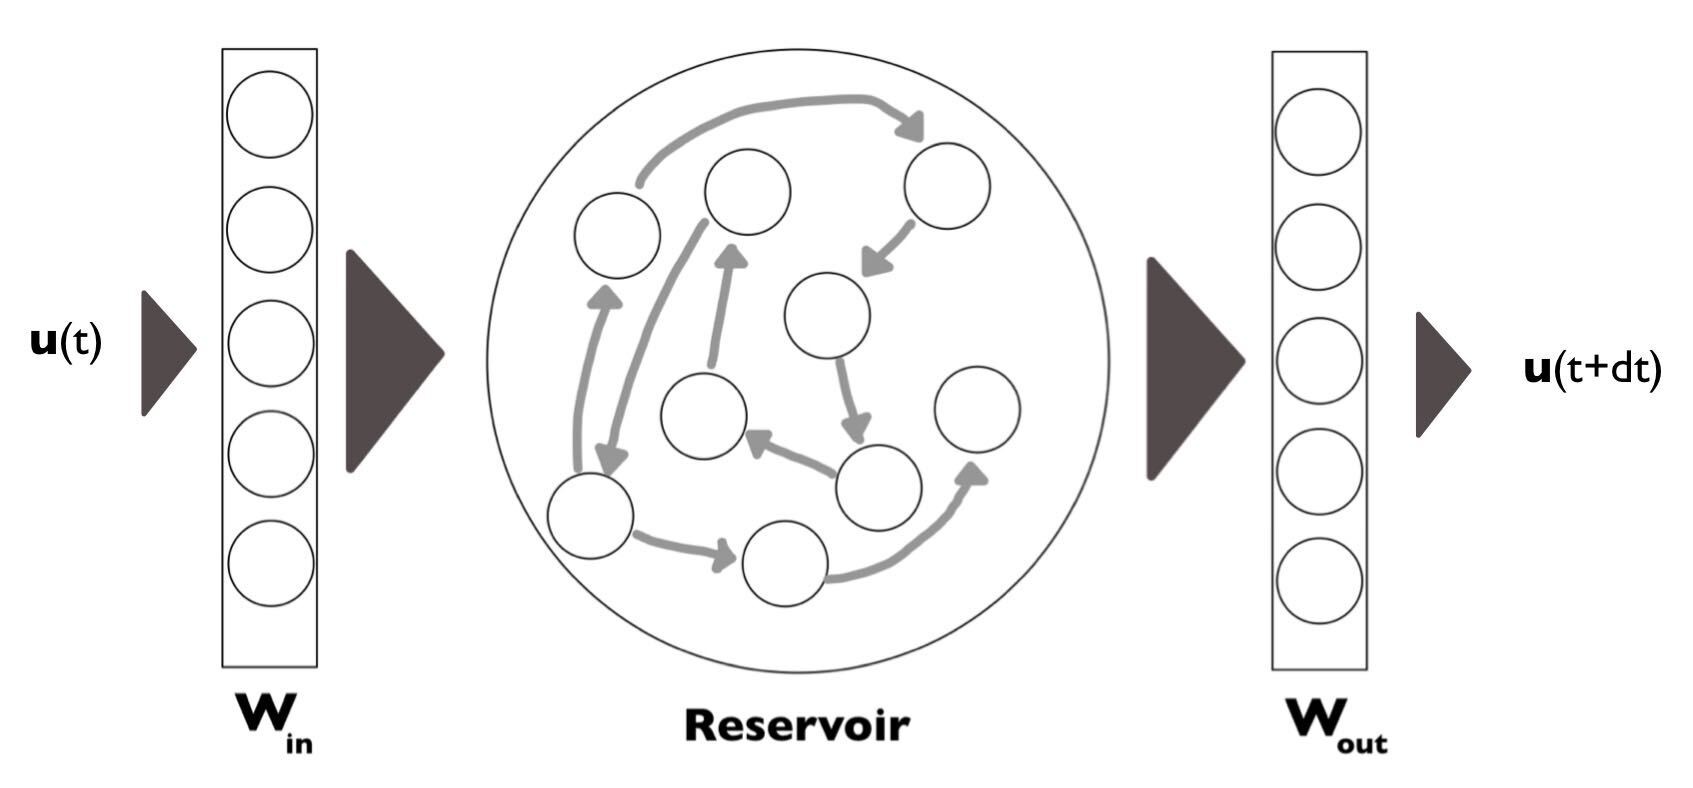
\includegraphics[width=\columnwidth]{reservoir_network.jpg}
	\caption{A basic reservoir computer or echo state network. The connections in
	the reservoir are given by $\bm{A}$}
	\label{fig:RCmodel}
\end{figure}

Figure \ref{fig:RCmodel} gives a visual representation of a basic
\acrshort{ESN}. An
input vector of length \textit{K} is mapped to the reservoir layer by an input
weight matrix $\bm{W_{in}}$. The state of the reservoir is mapped to an output
layer of length \textit{N} with an output weight matrix $\bm{W_{out}}$.
The output weight matrix is trained through
backpropagation using a loss function like cross entropy
\cite{pathak_model-free_2018, vlachas_backpropagation_2020}.

In this
work, the input vector is a function of time, $\bm{u}(t)$, and the output
vector is the next state of the system, $\bm{u}_p(t+\Delta t)$. Ideally, the
difference between the prediction, $\bm{u}_p$, and the actual, $\bm{u}_a$, is
minimized. \glspl{ESN} are capable of mapping an input vector of any size to
an output vector of any size. For example, $\bm{u}(t)$ could be the total
demand
at $t$ and $\bm{u}_p(t+\Delta t)$ could be the total demand at $t+\Delta t$. In
that scenario the reservoir is a one-to-one map. Alternatively, $\bm{u}(t)$
could be several data points, temperature, air pressure, irradiance, wind
speed, and total demand, at time $t$ and $\bm{u}_p(t+\Delta t)$ could be the
net demand at $t+\Delta t$. In this case the reservoir is a many-to-one map.
Determining the combination of input data that leads to the most accurate
predictions is a key area of research and an important part of this study
\cite{kobylinski_high-resolution_2020,bianchi_reservoir_2020}. For the results
shown below, $\bm{u}(t)$ is just the hourly demand.

\subsection{\textbf{Hyperparameter Search}}
Due to the architecture of \glspl{ESN}, the weights and connections
inside the reservoir do not need to be trained and, in our choice of
implementation, cannot be. This dramatically reduces the training time because
only the linear output layer needs to be trained. One drawback of this approach
is its sensitivity to hyperparameters, which must be carefully chosen before
running the network \cite{ pathak_model-free_2018,
lukosevicius_practical_2012, lukosevicius_reservoir_2009,gallicchio_deep_2019}.
Here, we perform grid searches
to establish which combination of hyperparameters minimizes the mean squared
error of the model,
\begin{align}
	MSE &= \frac{1}{N}\sum_i^N (\hat{y} - y_i)^2\\
	\intertext{where}
	\hat{y} &= \mbox{the average value of the ouput.}\nonumber
\end{align}

\subsection{\textbf{Constructing the \gls{ESN}}}

We constructed the \gls{ESN} in our initial demonstration with the open source
Python package \texttt{pyESN} \cite{korndorfer_pyesn_2015}. The code
is freely available on GitHub. Two models were trained with
historical demand data from \gls{uiuc} in 2017.  Each model had a
reservoir of 500 neurons. One was trained on 1000 hours of
data and predicted the following 100 hours of demand in two hour
increments. The other was trained on 3500 hours of data and, once again,
predicted the following 100 hours.

A grid search informed our choice of hyperparameters for these models, shown in
Figure \ref{fig:gridsearch}. This search determined the optimal combination of
spectral radius ($\rho$) and noise injection (for regularization of reservoir
neurons), shown in Figure \ref{fig:gridsearch}, following the recommendations
from \cite{lukosevicius_practical_2012}.

\begin{figure}[h]
  \centering
  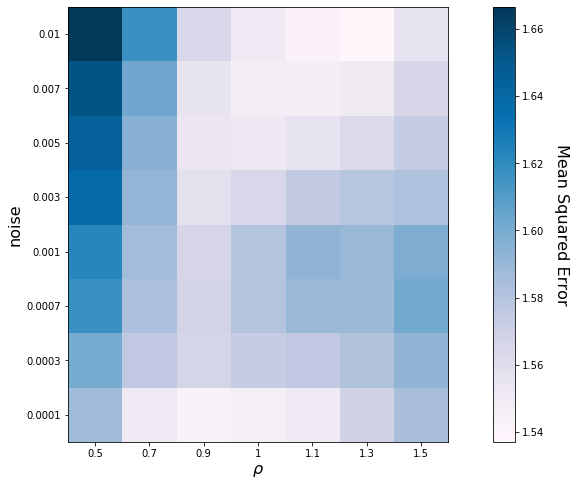
\includegraphics[width=0.8\columnwidth]{noise_spectral_radius.png}
  \caption{A grid search over a range of spectral radii and noise levels. The
  optimal set minimizes the mean squared error.}
  \label{fig:gridsearch}
\end{figure}


%%%%%%%%%%%%%%%%%%%%%%%%%%%%%%%%%%%%%%%%%%%%%%%%%%%%%%%%%%%%%%%%%%%%%%%%%%%%%%%%
\section{Results}
The first model, shown in Figure \ref{fig:ESN1}, we trained with 1000 hours of
historical data. The blue line is a snapshot of historical demand data. The
dashed line indicates the end of the model training and the beginning of the
model prediction. The red line is the prediction made by the \gls{ESN}. By
inspection, the \gls{ESN} successfully predicted a general
trend but had difficulty with accuracy at the desired hourly resolution.

\begin{figure}[h]
  \centering
  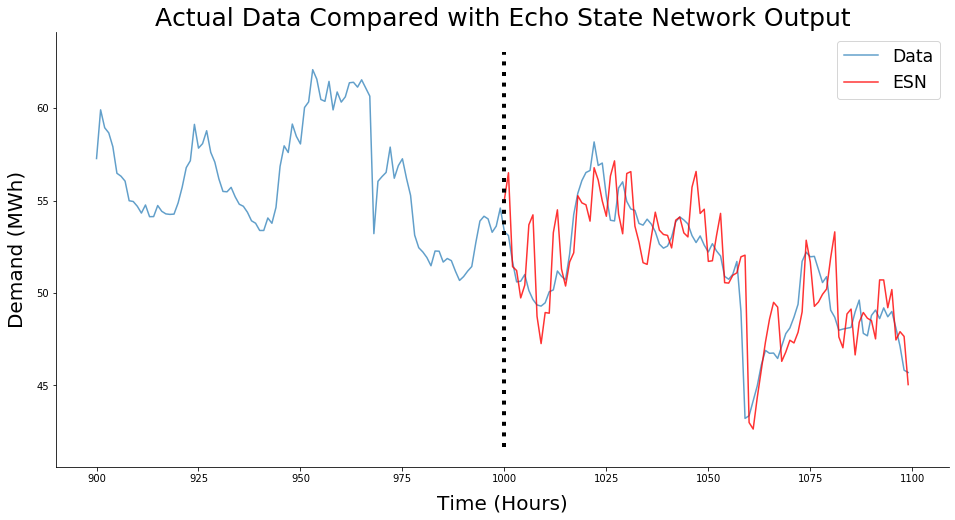
\includegraphics[width=\columnwidth]{scaled_esn_network2.png}
  \caption{A simple ESN with a prediction of 100 hours into the future after
  training on 1000 hours of historical data.}
  \label{fig:ESN1}
\end{figure}

The second model, shown in Figure \ref{fig:ESN2}, we trained with the same
dataset as before and extended the training to 3500 hours of
historical data. This \gls{ESN} made better predictions than the first model
and is most likely due to longer training. The effect of training
length on model accuracy will be explored in future work.

\begin{figure}[h]
  \centering
  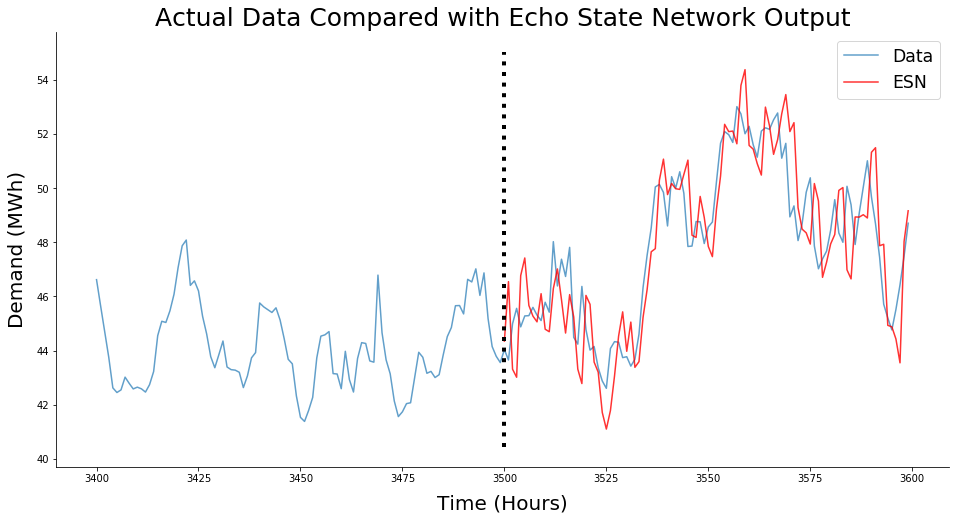
\includegraphics[width=\columnwidth]{scaled_esn_network.png}
  \caption{A simple ESN with a prediction of 100 hours into the future. After
  training on 3500 hours of historical data.}
  \label{fig:ESN2}
\end{figure}

Both models use training data with an hourly resolution. It is possible
that data at the 15-minute or 30-minute timescale will improve prediction
accuracy.


%%%%%%%%%%%%%%%%%%%%%%%%%%%%%%%%%%%%%%%%%%%%%%%%%%%%%%%%%%%%%%%%%%%%%%%%%%%%%%%%
\section{Conclusions}

We have demonstrated that even a basic \acrshort{ESN} can
predict the evolution of dynamic systems as others have
\cite{pathak_model-free_2018,wikner_combining_2020,bianchi_reservoir_2020}.
Future work will include:
\begin{enumerate}
  \item Identifying ideal input vectors, whether a single value for net demand
  history will suffice or some combination of values (e.g. local weather and
  total demand) will improve predictive power.
  \item Grid searches to tune hyperparameters.
  \item Taking advantage of fast model training to perform uncertainty analysis.
\end{enumerate}
Fairer comparisons on the effectiveness of training length will be done by
fixing the prediction time period for each ESN.
Accurate predictions of chaotic systems, like wind energy production, will
enable nuclear power plants to improve their economic feasibility through
relaxed load following.


%%%%%%%%%%%%%%%%%%%%%%%%%%%%%%%%%%%%%%%%%%%%%%%%%%%%%%%%%%%%%%%%%%%%%%%%%%%%%%%%
\section{Acknowledgments}

This work was made possible with data provided by UIUC
Facilities and Services, in particular, Morgan White, Mike Marquissee, and Mike
Larson. Additionally, this work is supported by the Nuclear Regulatory
Commission Fellowship Program.
Prof. Huff is supported by the Nuclear Regulatory Commission Faculty Development Program (award NRC-HQ-84-14-G-0054 Program B), the Blue Waters sustained-petascale computing project supported by the National Science Foundation (awards OCI-0725070 and ACI-1238993) and the state of Illinois, the DOE ARPA-E MEITNER Program (award DE-AR0000983), and the DOE H2@Scale Program (Award Number: DE-EE0008832)



%%%%%%%%%%%%%%%%%%%%%%%%%%%%%%%%%%%%%%%%%%%%%%%%%%%%%%%%%%%%%%%%%%%%%%%%%%%%%%%%
\bibliographystyle{ans}
\bibliography{bibliography}
\end{document}
